\documentclass[12pt, letterpaper, twoside]{article}
\usepackage{nopageno,epsfig, amsmath, amssymb}
\usepackage{physics}
\usepackage{mathtools}
\usepackage{hyperref}
\usepackage{xcolor}
\usepackage{array}
\hypersetup{
    colorlinks,
    linkcolor={blue},
    citecolor={blue},
    urlcolor={blue}
}
\usepackage{empheq}
\usepackage{wrapfig}

\usepackage[letterpaper,
            margin=0.8in]{geometry}

\newcommand{\psetnum}{8}
\newcommand{\class}{ASTR 541 - Interstellar Medium}

\newcommand{\tomtitle}{
    \noindent {\LARGE \fontfamily{cmr}\selectfont \textbf{\class}} \hfill \\[1\baselineskip]
    \noindent {\large \fontfamily{cmr}\selectfont Problem Set \psetnum \hfill \textsc{Tom Wagg}}\\[0.5\baselineskip]
    {\fontfamily{cmr}\selectfont \textit{\today}}\\[2\baselineskip]
}

\title{\class : Week \psetnum}
\author{\textbf{Tom Wagg}}

\newcommand{\question}[1]{{\noindent \it #1}}
\newcommand{\answer}[1]{
    \par\noindent\rule{\textwidth}{0.4pt}#1\vspace{0.5cm}
}
\newcommand{\todo}[1]{{\color{red}\begin{center}TODO: #1\end{center}}}

% custom function for adding units
\makeatletter
\newcommand{\unit}[1]{%
    \,\mathrm{#1}\checknextarg}
\newcommand{\checknextarg}{\@ifnextchar\bgroup{\gobblenextarg}{}}
\newcommand{\gobblenextarg}[1]{\,\mathrm{#1}\@ifnextchar\bgroup{\gobblenextarg}{}}
\makeatother

\newcommand{\avg}[1]{\left\langle #1 \right\rangle}
\newcommand{\angstrom}{\mbox{\normalfont\AA}}
\allowdisplaybreaks

\newcolumntype{C}{>{$}c<{$}}

\begin{document}

\tomtitle{}

\noindent For reference, if you'd ever like to see the code that I've used to get my answers to these, \href{https://github.com/TomWagg/uw-grad-classes/tree/main/541_ism}{here's a link to my GitHub repo}! (\#astropy.units for life)\\


\question{\textbf{1. Fun with the SiIV Doublet}}

\question{1a. An exercise in counting}
\answer{
    We have copies of each component of the SiIV doublet on graph paper. We can therefore use the grid to estimate the ratio of equivalent widths. No doubt this grid has physical meaning and units...but it'll just cancel I guess so I'm going to ignore that and just count boxes :D

    I find that the number of boxes for the 1402 is 14.5, and for the 1393 is 24. This gives that the ratio is
    \begin{equation}
        \boxed{ \frac{W_{1393}}{W_{1402}} = 1.66 }
    \end{equation}
}

\question{1b. Curve of Growth Regime}
\answer{
    We would expect this ratio to be 2 if we were in the linear regime. Given that it is a metal line, we can assume that it's not in the damped regime and so this means that it must be in the \textbf{flat} regime. This means that we must have some saturation in our measurement, which will lead to an underestimate of the column density!!
}

\question{1c. $\tau_0$ constraints}
\answer{
    If we assume that my measurement of the equivalent widths was perfect (doubtful), the equation in the question gives that
    \begin{align}
        \frac{W_{1393}}{W_{1402}} &= \qty[1 + \ln(f_{1393} \lambda_{1393}/f_{1402} \lambda_{1402}) / \ln(\tau_0 / \ln 2)]^{1/2} \\
        1.66 &= \qty[1 + 0.694 / \ln(\tau_0 / \ln 2)]^{1/2} \\
        \ln(\tau_0 / \ln 2) &= 0.4 \\
        \Aboxed{ \tau_0 &= 1.033 }
    \end{align}
}

\question{1d. AODM (not Another Ol' Dark Matter)}
\answer{
    I should actually write down that this means Apparent Optical Depth Method or I'll forget haha. Given that our line is saturated and has an optical depth above 1, this method will only give a \textbf{lower limit} on the column density
    \begin{align}
        N &= 1.13 \times 10^{7} \unit{cm^{-2}} \frac{W_{\lambda} (\unit{m\angstrom})}{f_{\lambda} \lambda^2(\unit{\angstrom})} \\
        N_{1393} &> 5.51 \times 10^{12} \unit{cm^{-2}} \\
        \Aboxed{ N_{1402} &> 6.62 \times 10^{12} \unit{cm^{-2}} }
    \end{align}
    where we've used that $W_{1393} = 50 \unit{m\angstrom}$ (from the question) and that $W_{1402} = 30.2 \unit{m\angstrom}$ (using the ratio we found).
}

\question{1e. Cloudy with a chance of Silicon}
\answer{
    We find a lower limit on the abundance of silicon as
    \begin{equation}
        12 + \log_{10}({\rm Si / H}) > 12 + \log_{10}\qty(\frac{10 \cdot 6.62 \times 10^{12}}{10^{19}}) > 6.82 \\
    \end{equation}
    This is lower than solar abundance and so this cloud likely formed from more metal-poor gas.
}

\question{1f. FWHM is back}
\answer{
    We can calculate $\sigma_{v, \rm turb}$ as
    \begin{align}
        \sigma_{v, \rm turb} &= \qty[\frac{\rm FWHM^2}{8 \ln 2} - \frac{k_B T}{M}]^{1/2} \\
        \sigma_{v, \rm turb} &= \qty[\frac{\rm (40 \unit{km}{s^{-1}})^2}{8 \ln 2} - \frac{k_B \cdot 10000 \unit{K}}{1 \unit{amu}}]^{1/2} \\
        \Aboxed{ \sigma_{v, \rm turb} &= 14.35 \unit{km}{s^{-1}} }
    \end{align}
    If we assume that the temperature is the same, we would assume that the FWHM of the Silicon would be
    \begin{equation}
        {\rm FWHM}_{Si} = \sqrt{8 \ln 2 \qty[\sigma_{v, \rm turb}^2 - \frac{k_B T}{28 \unit{amu}}]} = 34 \unit{km}{s^{-1}}
    \end{equation}
    If we instead measure $50 \unit{km}{s^{-1}}$ then it may be possible that our assumption of equal temperatures was not valid.
}

\question{\textbf{2. The Grand Return of Xspec GUI}}

\question{2a. Favourite Systems}
\answer{
    \begin{center}
        \begin{tabular}{c|c|c}
            Redshift, $z$ & Shows SiIV? & Shows OVI? \\
            \hline\hline
            0.1470 & \checkmark & $\times$ \\
            0.2055 & \checkmark & \checkmark \\
            0.2180 & $\times$ & \checkmark \\
            0.35566 & $\times$ & $\times$
        \end{tabular}
    \end{center}
    In the cases in which there was no absorption, it is either because (i) the ratio of EWs is reversed, implying another species is interfering sneakily (ii) the line is redshifted outside of the observed wavelength range (iii) there was just no change in normalised flux.\\

    \noindent \textbf{My favourite system is at $\mathbf{z = 0.35566}$}, its lack of both SiIV and OVI absorption lends it an air of mystery and wonder that is unparalleled amongst the other systems. Alas, I have doubts about its continued involvement in the remainder of the problem, so long $z = 0.35566$!
}

\question{2b. OVI Doublet}
\answer{
    Using the GUI I find that the OVI doublet EW ratios are
    \begin{center}
        \boxed{\begin{tabular}{c|c}
            Redshift, $z$ & OVI Ratio \\
            \hline\hline
            0.2055 & 1.30 \\
            0.2180 & 1.58
        \end{tabular}}
    \end{center}
    Since both of these ratios are less than 2 (the expected ratio for the linear regime) and there is no evidence of strong lorentzian wings, this implies that both are in the \textbf{flat regime of the curve of growth}.
}

\question{1c. Curve of Growth}
\answer{
    Here's my curve of growth! We can see that the Silicon tends to be closer to the linear regime but it swerves off towards the flat part. The first HI line is possibily still in the flat part but after that is seems to rise following the square root regime.
    \begin{center}
        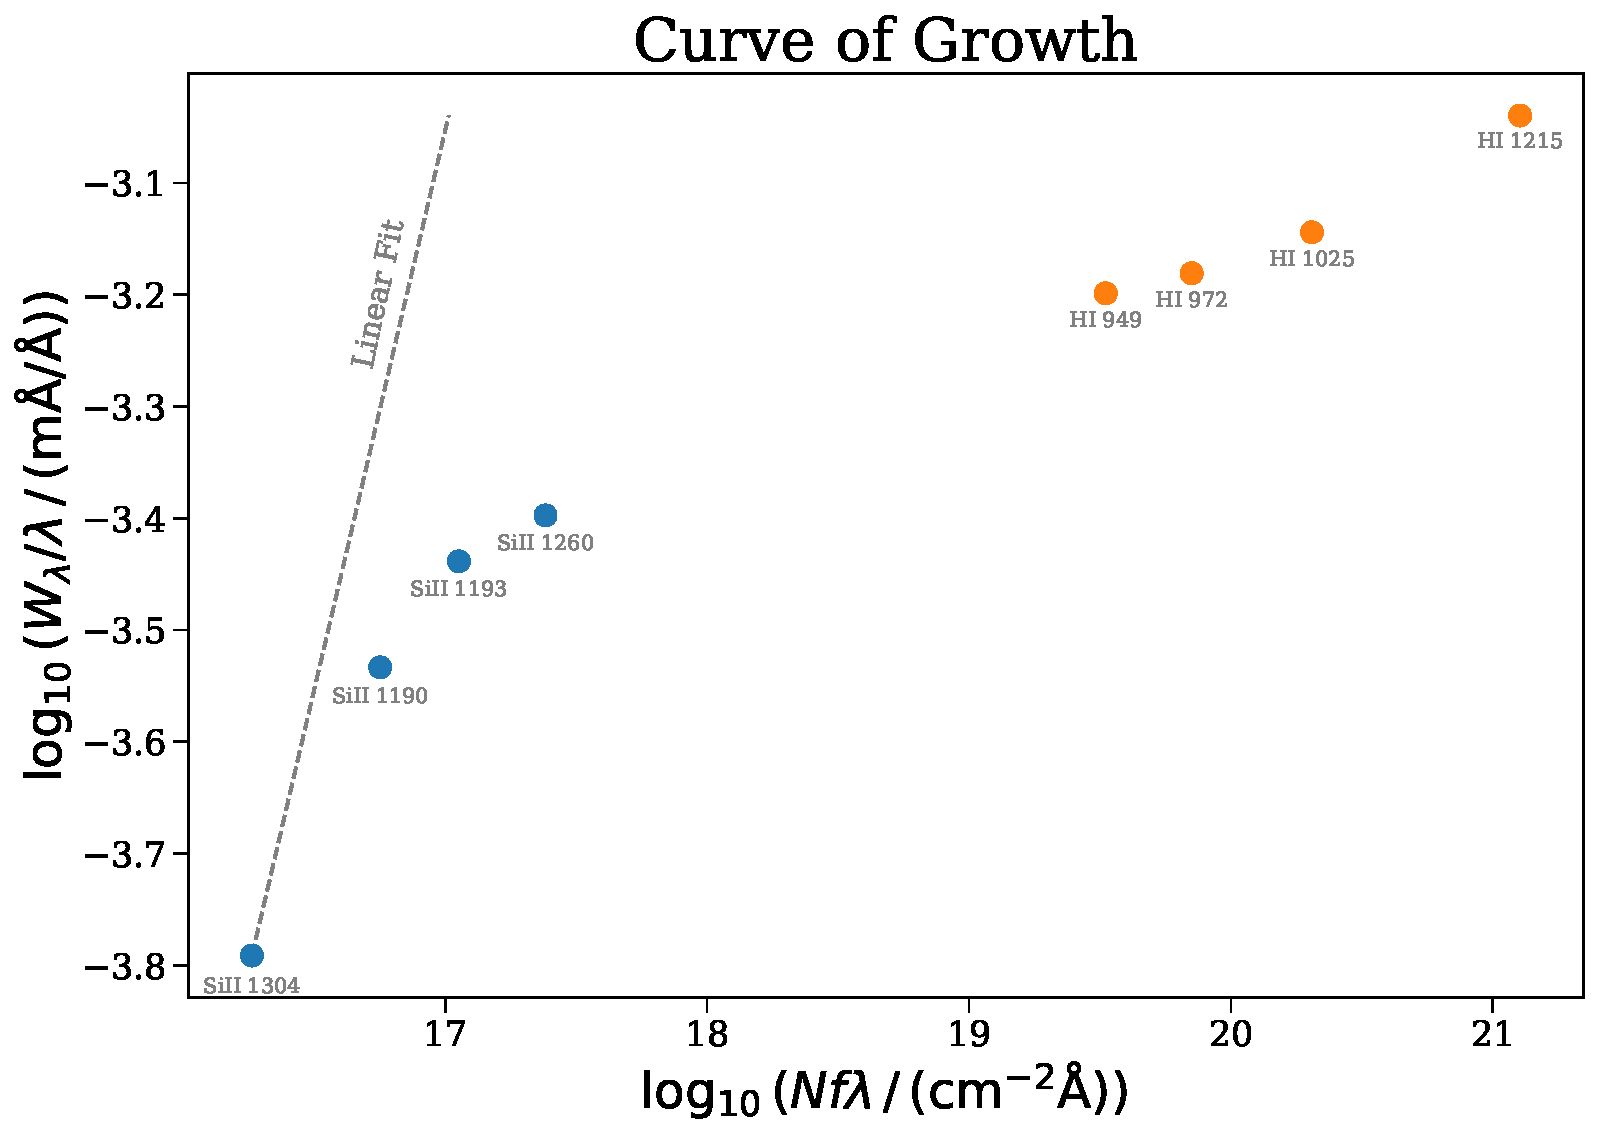
\includegraphics[width=0.8\textwidth]{cog.pdf}
    \end{center}
    Absorption line saturation can be contextualised as diverging from the linear part of the curve of growth and heading into the flat part I think.
}

\end{document}

 